\chapter{Introduction}

\section{Generative Models}
\label{sec:intro_generative_models}

\begin{quote}
	What I cannot create, I do not understand - Richard Feynman
\end{quote}

\begin{figure}[ht!]
	\centering
	\begin{tabular}{cc}
		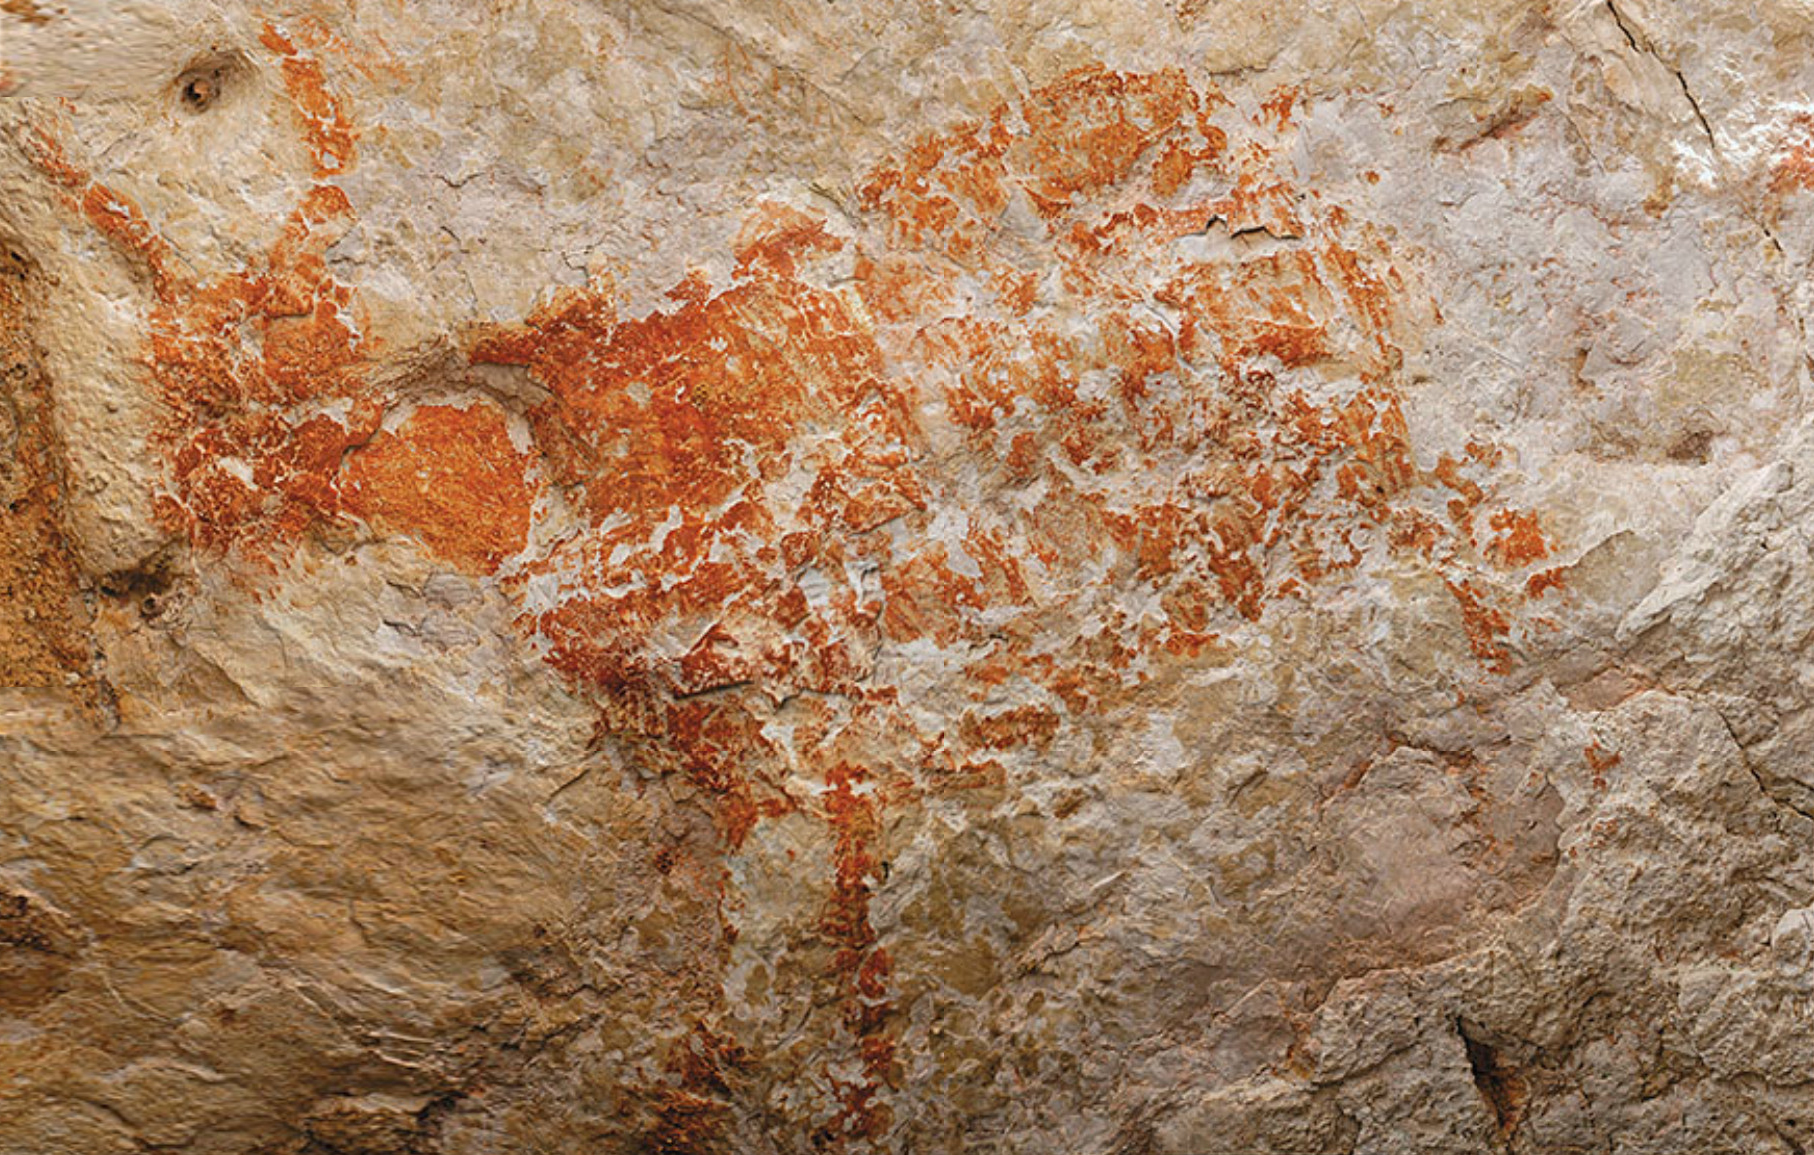
\includegraphics[width=0.49\linewidth]{figures/intro/cave_painting_of_bull.jpeg} &
		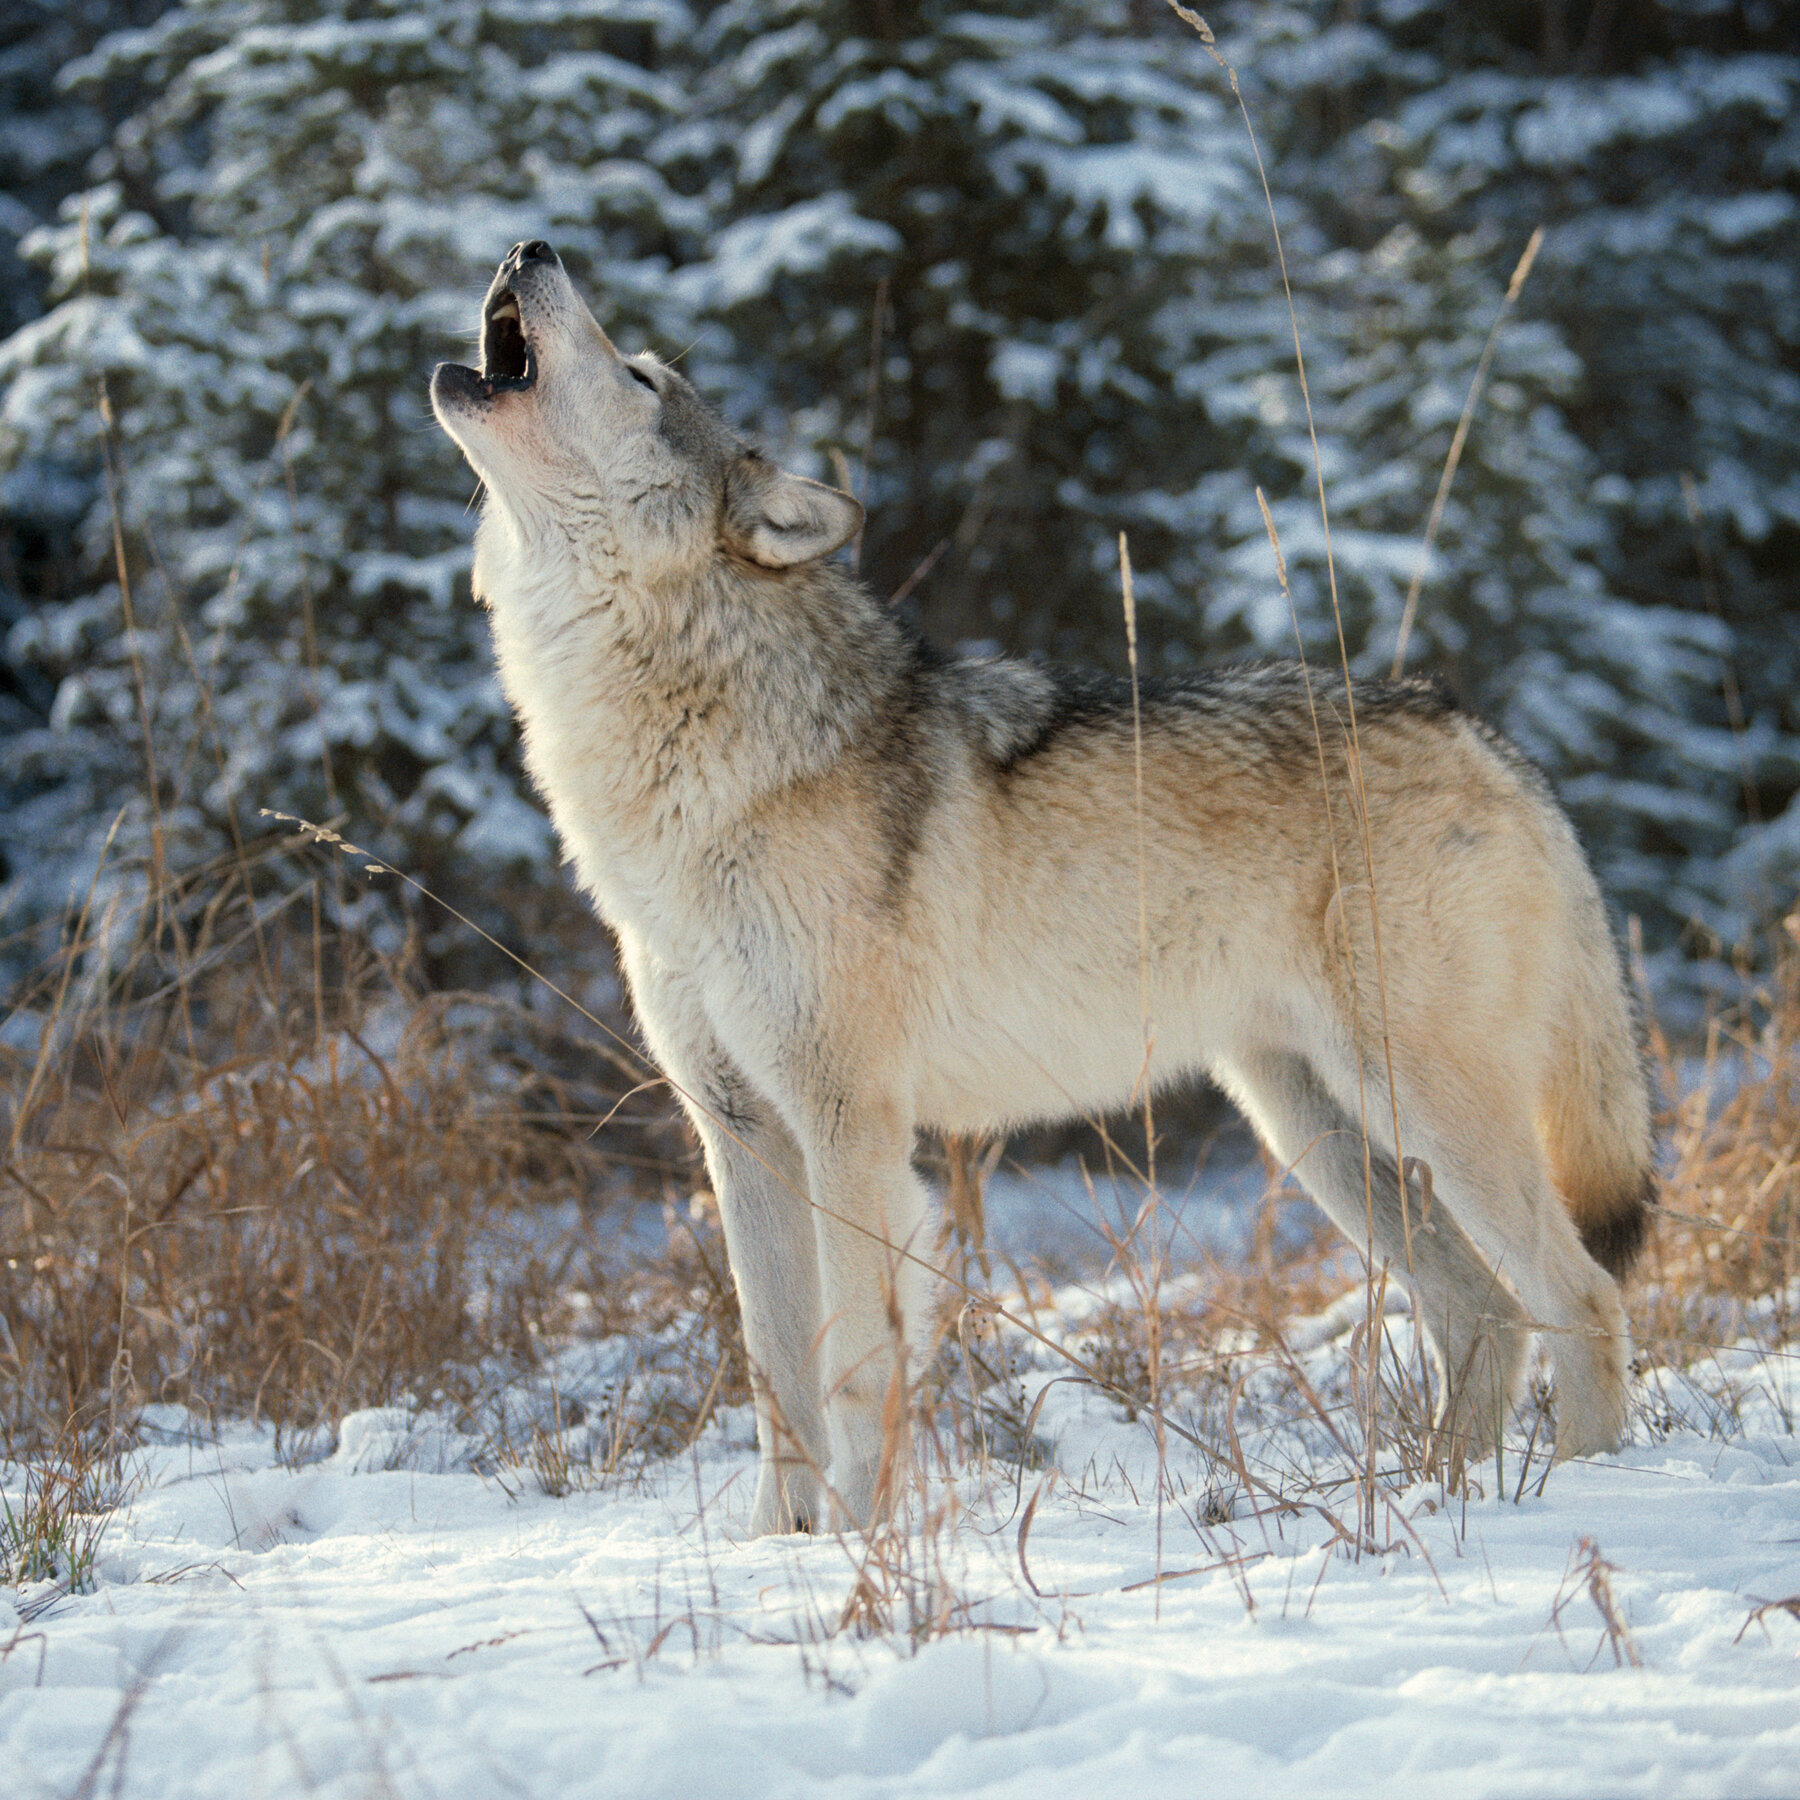
\includegraphics[width=0.31\linewidth]{figures/intro/wolf_nyt.jpeg}
		\\
	%(a) One of the oldest known figurative paintings, a depiction of an unknown bovine, was discovered in the Lubang Jeriji Saléh cave and dated to be more than 40,000 (perhaps as old as 52,000) years old. & (b) Recent photograph of a wolf from New York Times
	\end{tabular}	
	\caption[Efficacy of visual communication]{
		We are able to recognize the bovine creature almost as succinctly as we understand the wolf. However if we're magically transported to the past when this was being painted we wouldn't understand any of the language being spoken.
		}
	\label{fig:cave_painting}
\end{figure}

Visual communication had been the primary method of communication since time immemorial. If we go back to some of the earliest known cave paintings more than 10,000 years ago, we would still recognize what they were trying to communicate. As seen in Figure \ref{fig:cave_painting}. Language evolved in humans as a form of communication since the tools to communicate visually were non ubiquitous. If a wolf was nearby and someone started drawing it would already be too late to save anyone.

The tools at the time didn't enable us to draw a wolf fast enough to stop us from being eaten. Thus humans invented language as a means to communicate. If we suddenly invent a time machine and go back thousands of years to the caves with the earliest cave paintings, we would still understand the bull and the impending danger to the human settlement. However if we try to communicate in either English or any other modern language with the prehistoric cave dwellers neither of us would be able to communicate with the other. However, if we showed them a TikTok video of another human, even the prehistoric cave dwellers would most likely be able to identify with the emotions shown in the video. 

\paragraph{Language  as  a bottleneck}
Language along with the immense benefits which depends upon a shared context has as its achilles heel the same thing which makes it most powerful: shared context. When we talk about our Italian holiday, it can mean so many different things to different people. Some would focus on the feel of the air, others on the mediterranean weather. Others on piazzas. Some would envision the passion for the Ferrari F1 team while others might imagine the obvious taste of the delicious pizzas. All of the above is compressed in a single phrase titled "Italian holiday".

\paragraph{Why is visual communication important}

\begin{itemize}
	\item \textbf{Expressing Emotions:} are hard to express via text on the internet
	
	\item \textbf{Saves time:}
	
	\item \textbf{Promotes consistency:}
	
	\item \textbf{Provides Clarity:}
	
	\item \textbf{Increases retention:}
	
	\item \textbf{Universally understood:}
	
	\item \textbf{More impactful:}
	
\end{itemize}


\paragraph{Current state of the art in Visual Communication for mere mortals}

GIFs are the go to medium for expressing our emotions at the moment. Platforms such as Instagram, snapchat and Tiktok have changed how we communicate visually. Tiktok allows us to make videos which would have taken hours of work on Adobe Premier Pro. Instagram and the modern smartphone cameras have rendered the bulky DSLRs obsolete. We now have Google Lens which can identify anything you don’t know in a matter of seconds. 

\paragraph{Future of visual communication}

Interesting products coming to the forefront. Interactive product design in Virtual reality via the oculuses and the holo lenses of the world. 
Just like when you search “How to” on google, and it starts suggesting “how to give a swashbuckling speech on Toastmasters”. Products from Adobe are coming up which starts autocompleting your sketches and also photo-realisitically renders it.
So with a few strokes of your stylus you can design \& customise  your own luxury sports car or your new set of fancy boots.
 In the future when you can 3D print items, you can quickly design your stuff assisted with Ai and just 3D print it at home. When you watch a movie, you’d like to see yourself as the protagonist on the top of Burj Khalifa rather than Mr Tom Cruise. Ads in the future would feature you in that Armani suit and give you serious FOMO leading your Fear to buy that Armani suit or dress.

The tools for visual communication are becoming an even faster media of communication than traditional forms of text. It thus becomes imperative to design the future of visual communication tools enhanced by data driven learning approaches. Generative models learn the underlying generative function that best fits the data. Once a generative model is trained it should ideally support generation of new samples from the underlying data distribution. 

Generative models spearheaded by Generative Adversarial Networks \cite{goodfellow2014generative} and Variational Autoencoders \cite{kingma2013auto} introduced applications which previously had been deemed impossible. 


\section{Taxonomy of Generative Models}

\begin{figure}
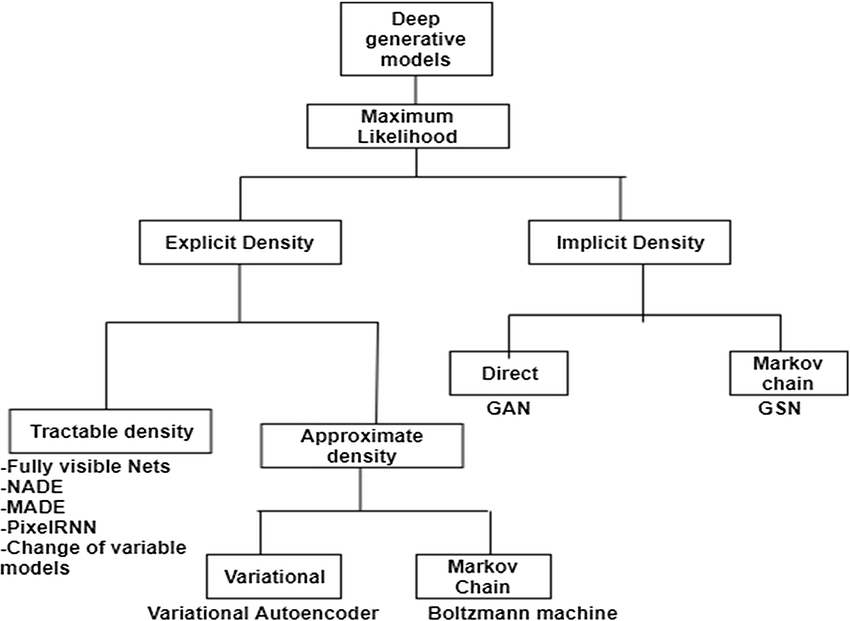
\includegraphics[width=\linewidth]{figures/intro/taxonomy-generative-models.png}
\caption{Taxonomy of Generative Models}
\label{fig:taxonomy_generative_models}

\end{figure}


Typical generative models are trained with maximum likelihood learning. The learnt density function can either be implicit as in the case of Generative Adversarial Networks\cite{goodfellow2014generative} and Generative Stochastic Networks \cite{alain2016gsns}. On the other hand the density can be explicitly modeled. Variational Autoencoders \cite{kingma2013auto} approximate the density function using the Evidence Lower Bound (ELBO). In case of autoregressive models such as PixelRNN\cite{van2016pixel} the density is tractable. Continuous Normalizing Flows \cite{chen2018neural, grathwohl2018ffjord} is also a form of explicit density estimation technique. 


Deep generative models models are function approximators, parametrized by a neural network with several layers. These networks are trained to approximate a complicated high dimensional probability distribution. On successful training, these trained models could either be used to estimate likelihood of a particular sample under the distribution. The trained deep generative model often allows us to draw samples from the distribution. Deep generative models has been one of the most active areas of research in recent years because of its incredible promise. Although, the promise hasn't been fulfilled and hence the increased research interest. In recent years three major avenues of deep generative model has taken centre-stage amongst many others. Variational Autoencoders(VAEs), Normalizing Flows(NFs) and Generative Adversarial Networks(GANs) are the ones that have shown the highest quality results. These are the models which have shown the highest resolution which can be potentially used for effective and reliable Visual Communication applications. 
 

\section{Applications of Generative Models for Visual Communication}
% Flesh it out with a bunch of images (wink visual communication)



\section{Challenges before Generative Models can become ubiquitous} 


\subsection{ Mode Collapse in GANs}

\subsection{ Improper Conditioning in Class Conditional GANs}

\subsection{ Assistance in Human Creativity}

\subsection{ Extremely slow training in Continuous Normalizing Flows}

\section{Approach}

\section{Structure of the thesis}
